\section{Experiments}
We have proceed to do an evaluation for experiments part.\\
First, we choose the dataset from Kaggle which is \textbf{Customer Rating Data By Amazon}. It can be found via \url{https://www.kaggle.com/datasets/ahmedaliraja/customer-rating-data-by-amazon/data} .Let's have the overview about dataset:\\
\\
%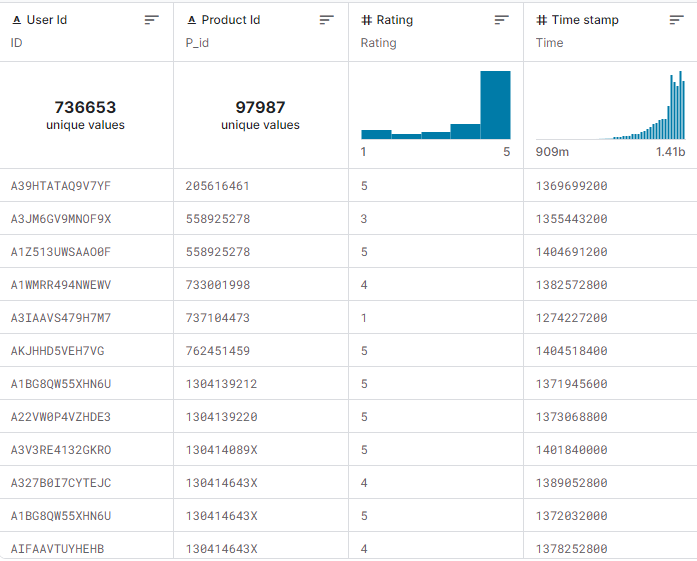
\includegraphics[scale=0.6]{image/dataset.png}
\\
\\
It comprises an extensive collection of over 2 million customer reviews and ratings of beauty-related products available on Amazon's platform. The dataset includes valuable information such as:
\begin{itemize}
    \item Unique User IDs for customer identification.
    \item Product ASIN (Amazon's distinctive product identifier).
    \item Ratings, which reflect customer satisfaction on a scale from 1 to 5.
    \item Timestamps, recorded in UNIX time, indicating when the ratings were submitted.
\end{itemize}
\indent  We did a small test on running 3 different algorithms and have the result as below:
\begin{figure}
    \centering
    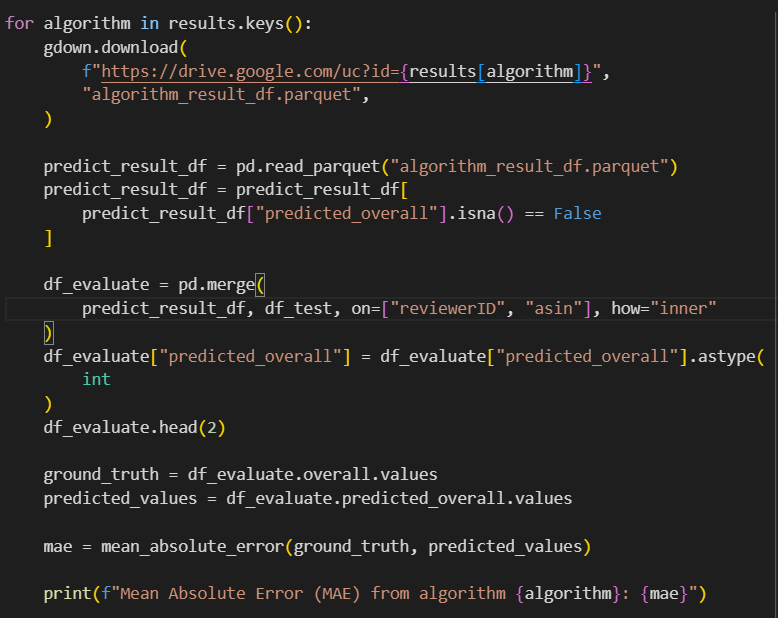
\includegraphics[scale = 0.6]{image/evaluation.png}
    \caption{Evaluation code with 3 different algorithms}
    \label{fig:enter-label}
\end{figure}
\\
\indent For the Mean Absolute Error (MAE) - 
The Mean Absolute Error (MAE) values provided for three different algorithms (Louvain, Label prop, and Greedy modularity) represent the average absolute differences between the predicted values and the actual values. : \\ \\
+ Louvain Algorithm: 1.3076923076923077 \\
This algorithm has a moderate MAE, suggesting that its predictions have a moderate level of error on average.\\
\\
+ Label prop Algorithm: 1.75 \\
This algorithm has a higher MAE compared to the Louvain Algorithm, indicating that, on average, its predictions have a larger error.\\
\\
+ Greedy modularity Algorithm: 1.125984251968504 \\
This algorithm has the lowest MAE among the three, suggesting that it provides more accurate predictions compared to the other two algorithms in your test.\\
\\
\indent In summary, based on the MAE values, the Greedy modularity Algorithm seems to perform the best among the three algorithms you tested, as it has the lowest MAE. 
